% 2024年北京高考数学第19题解析图1：椭圆与交点几何
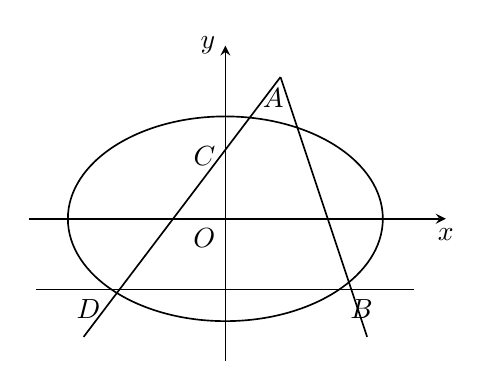
\begin{tikzpicture}[>=stealth,line width=0.6pt,font=\normalsize]
  \draw[->] (-2.5,0) -- (2.8,0) node[below] {$x$};
  \draw[->] (0,-1.8) -- (0,2.2) node[left] {$y$};
  \node[below left] at (0,0) {$O$};

  % 椭圆
  \draw (0,0) ellipse (2.0 and 1.3);

  % 水平割线 y = -0.9
  \draw (-2.4,-0.9) -- (2.4,-0.9);

  \coordinate (D) at (-1.46,-0.9);
  \coordinate (B) at (1.46,-0.9);
  \coordinate (A) at (0.35,1.28);
  \coordinate (C) at (0,0.8);

  % 割线与三角形
  \draw (-1.8,-1.5) -- (0.7,1.8);
  \draw (0.7,1.8) -- (1.8,-1.5);

  \node[above right] at (A) {$A$};
  \node[below right] at (B) {$B$};
  \node[left] at (C) {$C$};
  \node[below left] at (D) {$D$};
\end{tikzpicture}
